\chapter{Evaluierung}
\label{ch:S6_Evaluierung}

\section{Qualität der Lösung}
\label{ch:CH6_qualtiy_of_solution}

Für eine Evaluation der in Kapitel \ref{ch:S4_Lösungsansatz} und \ref{ch:S5_Umsetzung} vorgestellten Lösung muss zunächst die Evaluationsmethode definiert werden. Für die Evaluation soll die Lösung der Arbeit mit der Problemstellung in Kapitel \ref{ch2:Problemstellunug} gegenübergestellt werden. Es wird untersucht inwiefern das Framework und das Beispiel Spiel zu einer Lösung der Problemstellung beitragen. Das Ergebnis der Evaluation soll entsprechend weitere Handlungsempfehlungen bzw. Verbesserungsvorschläge aufzeigen, sofern diese aufgrund der Evaluation notwendig sein sollten. 
Die vorgestellte Lösung soll im Hinblick auf die vier Hauptaspekte untersucht werden:

\begin{itemize}

\item Gamification unter Einbezug der Händler
\item Pervasive Games
\item Relokalisierbarkeit
\item Verwendbarkeit von OSM Daten

\end{itemize}

Die Evaluation der durch das Framework erzeugten Spielfelder und somit eine Bewertung der Relokalisierbarkeit wird in Kapitel \ref{ch:CH6_qualtiy_of_gameboards} behandelt.


\subsection*{Gamification}

Im Bezug auf die in Kapitel \ref{ch1:Einleitung} aufgestellte Motivation, soll die Lösung mittels Gamification den regionalen Händlern zu neuen Kunden führen können und bestehende entsprechend halten. Ziel ist es nicht zu überprüfen, ob und wie hoch der entsprechende Neukunden und Bestandskundenanteil durch die Lösung beeinflusst wird, sondern inwiefern entsprechende Elemente aus der Literatur umgesetzt wurden. Diese wiederum sollen die Möglichkeit für einen besseren Umsatz der Händler bieten.
In der Literatur wurden zunächst die rudimentären Elemente eines Gamification Prozesses herauskristallisiert. Für die softwaretechnische Umsetzung wurden bei der Implementierung die Anforderungen entsprechend umgesetzt, damit die Gamification-Elemente Points, Badges und Leaderboards problemlos verwendet werden können. Zudem wurden die Aspekte der klassischen Spieltheorie aufgegriffen und dadurch die Gamificationen Ansätze erweitert. Es wurden mehrere Optionen aufgezeigt, welche in Spielen umgesetzt werden können. Darüber hinaus wurden diese Aspekte mit entsprechenden Technologien wie NFC oder Bluetooth Low Energy in Verbindung gebracht, wie eine Integration der Spielelemente vor Ort bei den Händlern gestaltet werden könnte. Das Framework und das Beispiel Spiel bilden diese nicht alle ab, sind aber problemlos in der Funktionalität erweiterbar.
Durch die Kombination der Gamification Elemente und der Generierung von Spielelementen auf Basis der Umgebung in Kombination der lokale Händler wird das Maß der Immersion für die Spieler erhöht und der Effekt der Gamification verstärkt.
Für den Aspekt der Gamification lässt sich daher abschließend festhalten, dass die aufgezeigte Lösung einen Beitrag zur Lösung der Problematik der Gamification von Neukundenbesuchen bei regionalen Händlern liefern kann.

\subsection*{Pervasive Games  -- Anforderungen an ein Gameframework}

Im Zuge der Erstellung eines Frameworks zum Staging von Pervasive Games müssen mehrere Aspekte behandelt werden. Zunächst muss definiert werden, welche Grenzen des Magic Circle überschritten werden. Im Zuge dieser Arbeit lag der Fokus auf der Dimension Ort und Zeit. Das bedeutet, dass ein entsprechendes Spiel soll sowohl ortsunabhängig als auch zeitunabhängig gespielt werden kann. Die Ortsunabhängigkeit der vorgestellten Lösung wird durch die Relokalisierung mit Hilfe von OSM-Daten sichergestellt. Die zeitliche Unabhängigkeit ist dadurch sichergestellt, dass jeder Spieler sich individuell am Beispiel Spiel anmelden kann und es keine fest definierten Uhrzeiten oder Termine gibt um das Spiel zu spielen. Im Vergleich zu typischen Geogames ist es daher möglich auch über feste Uhrzeiten und Geografische Gebiete hinaus das Spiel zu spielen. Durch die entsprechende Formulierung der Anforderungen in Kapitel \ref{ch2:Problemstellunug} und \ref{ch4:s:Lösungen} und der Ausrichtung des Frameworks an diesen wurde sichergestellt, dass das Framework diese Anforderungen erfüllt. Da es sich in der Problemstellung um ein Echtzeitspiel handelt muss auch entsprechend im Framework sichergestellt werden, dass die Interaktion mit dem Spiel in Echtzeit erfolgen kann.
Durch die Modularisierung und Auskopplung der Evaluation der OSM Tags, ist es möglich die zeitintensiven Bewertung der Spielfelder unabhängig von der Spielfeldgenerierung durchzuführen. Dadurch ist wird es möglich, lediglich die relativ einfachen Prozesse zur Transformation der OSM-Elemente während der Laufzeit durchzuführen. Vergleicht man die durchschnittliche Antwortzeit des Frameworks, so ist diese ausreichend niedrig. Die Varianz ist wie in Abbildung \ref{img:ch6_img01_response_time} erkenntlich zu vernachlässigen.  Die Antwortzeit ist  abhängig von der Anzahl der OSM-Elemente in der Bounding Box und der Antwortzeit des Overpass API Servers, jedoch steigt diese nicht weiter, wenn die empfohlene maximale Anzahl an Spielelementen nicht überschritten wird. Die Evaluationsfunktion hingegen liegt bei 2-3 Minuten für ein Tag mit ca. 200 Elementen. Für ein Feld mit 1200 Elementen liegt diese bereits bei über 30 Minuten.

\begin{figure}[H]
\begin{center}
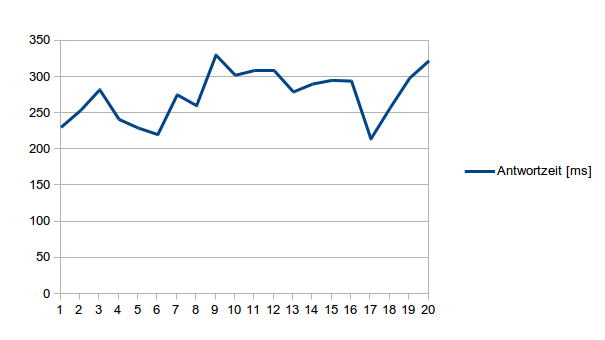
\includegraphics[width=150mm]{images/ch6_img01_response_time.png}
\caption{Antwortzeit der GameAPI für den Tag public\_transport = stop\_area}
\label{img:ch6_img01_response_time}
\end{center}
\end{figure}

Abweichungen der Antwortzeit sind weniger bedeutend, da das Spielfeld sich bereits vorher für den Spieler aufbaut und die Spielelemente mittels Ajax Request geladen werden. Darüber hinaus wird durch die dynamische Erweiterung der Bounding Box sichergestellt, dass alle Elemente am Rand der Karte bereits geladen sind. Das Nachladen der Elemente beim Fortbewegen kann daher auch minimal länger dauern, da das Spielfeld immer zentriert auf den Spieler ist.

Durch die Kapselung der einzelnen Module wird auch sichergestellt, dass eine Erweiterbarkeit der Spielmechanik ohne größeren Aufwand möglich ist. Das entsprechende Beispiel Spiel kann problemlos erweitert werden oder aber durch ein beliebiges anderes Spiel ersetzt werden.
Hierbei zeigt sich, dass die Anforderung für die Flexibilität des Frameworks hinsichtlich seiner Erweiterbarkeit und Austauschbarkeit gegeben ist.

\subsection*{Relokalisierbarkeit}

Der nächste essentielle Aspekt der Problemstellung war die Relokalisierbarkeit. Ziel war es im Zuge des zu vereinfachenden Stagings dem Spielleiter entsprechend eine Möglichkeit an die Hand zu geben, welche im auch ein Spielen außerhalb eines festen Bereiches ermöglicht. Hierzu wurden entsprechende OSM-Daten verwendet die durch eine Transformation zu Spielelementen umgewandelt wurden. Durch die entsprechende Evaluation der OSM-Tags im Voraus wird sichergestellt, dass der jeweils beste Tag für die getesteten Umgebungen ausgewählt wurde.
Die Transformation der OSM-Elemente funktioniert problemlos, speziell auch mit Relationen und Ways, wie in Abbildung \ref{img:ch6_img02_transform} zu erkennen ist. Auf der linken Seite sind die Daten aus OSM respektive Overpass zu sehen. Auf der rechten Seite sind hingegen die vom Framework erzeugen Spielelemente ersichtlich.


\begin{figure}[H]
\begin{center}
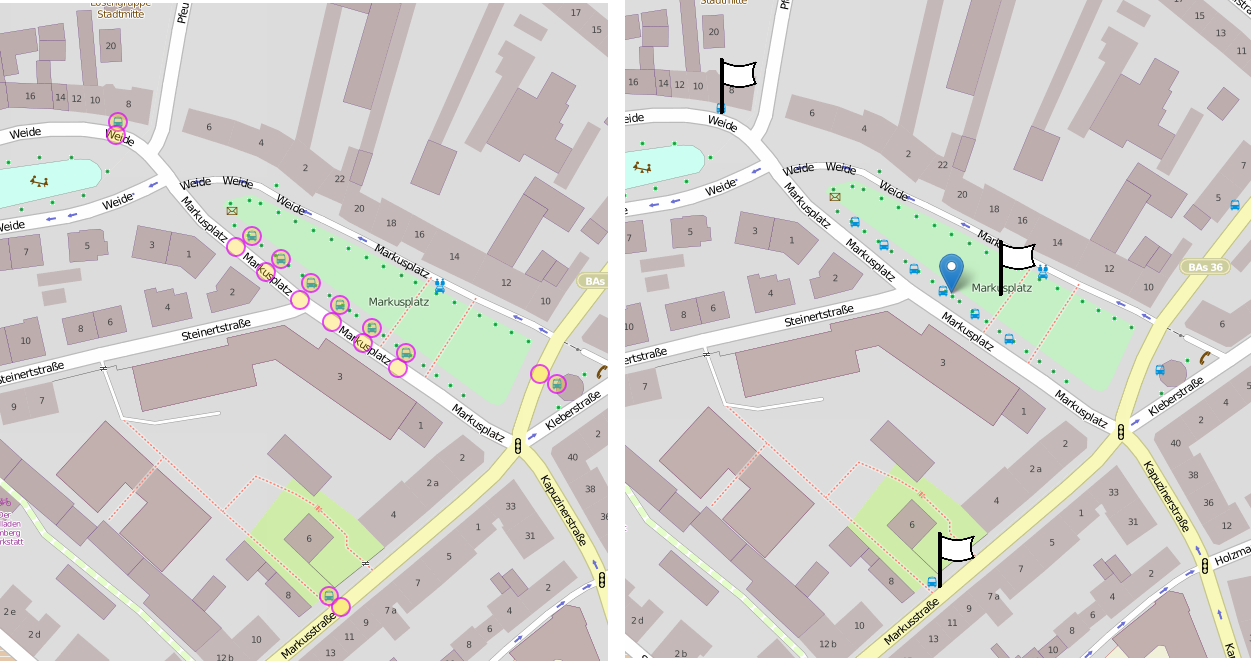
\includegraphics[width=150mm]{images/ch6_img02_transform.png}
\caption{OSM-Daten im Vergleich zu den transformierten Spielelementen}
\label{img:ch6_img02_transform}
\end{center}
\end{figure}

Sofern eine entsprechende Evaluierung im Voraus sichergestellt wurde, sind die Spielfelder ohne Einschränkungen nutzbar.
Einen Nachteil der Fokussierung auf ein einzelnes Key-Value Paar in OSM, ist die Möglichkeit, dass es z.\,B. in Regionen in denen eine geringere Mapping Qualität vorliegt, im Extremfall keine Spielelemente zur Verfügung stehen könnten. Diese Problematik könnte in diesem Fall durch eine einfache Anpassung des Frameworks gelöst werden. Hierzu müsste intern eine Liste mit alternativen Tags vorgehalten werden. Diese Liste könnte dynamisch auf Basis von \url{http://taginfo.openstreetmap.org/tags} gefüllt werden. Beim Aufruf der GameAPI müsste das Framework nur die vorhandene Zahl der Spielelemente prüfen und bei einer Unterschreitung eines vordefinierten Wertes automatisch den nächsten alternativen Tag verwenden. Zwar führt dies dazu, dass potentiell die Auswahl der Spielelemente für den Spieler schwerer nachvollziehbar ist, jedoch würde dies sicherstellen, dass auch im Worst Case Szenario entsprechend ausreichend Spielelemente generiert werden.

Somit lässt sich feststellen, dass die Relokalisierung problemlos funktioniert und auch entsprechend für den Einsatz mit Pervsaive Games geeignet ist. Ein offener Punkt ist eine weitere Optimierung für das Worst Case Szenario für den Fall, dass der optimale Tag im lokalen Bereich keine Spielfelder liefern kann.

\subsection*{Verwendbarkeit von OSM Daten}

Eine Fragestellung zu Beginn der Arbeit war die Verwendbarkeit von OSM Daten im Zuge von Pervasive Games.
Die Anforderungen an die Daten im Vergleich zu einer Navigationssoftware sind beim Framework vergleichsweise gering.
Es muss eine korrekte Klassifikation stattfinden und die Abweichung der Position sollte vorzugsweise nicht mehr als der Aktionsradius des Spielers betragen. Dadurch wird erreicht, dass alle Spielelemente auch entsprechend von den Spielern physisch erreichbar sind.
Fehler bei der Klassifikation können vorkommen, da es immer der Fall sein kann, dass die Daten nicht entsprechend korrekt gemappt wurden.
Dies ist aber im Zusammenhang des Frameworks nicht weiter relevant, da deswegen maximal das entsprechende Element/Objekt nicht auf dem Spielfeld erscheinen wird. Durch das Fehlen wird aber die Funktionalität des jeweiligen Spieles selbst nicht beeinträchtigt. Hierdurch wird lediglich die Verteilung auf dem Spielfeld beeinflusst. Probleme mit dem Spielfeld bei zu wenig Elementen wurden bereits angesprochen und mögliche Lösungen aufgezeigt.
Die Transformation der OSM-Daten stellt sicher, dass auch Mapping Fehler, z.\,B. das rekursive Verweisen von Relations, keine Probleme entstehen. Es wird sichergestellt, dass in jedem Fall die Transformation stattfindet.
Abschließend ist festzuhalten, dass OSM ohne Einschränkungen nutzbar ist.
Gründe hierfür sind die Ergebnisse in der Literatur, welche OSM eine ausreichende Datenqualität zusprechen und OSM auch hinsichtlich der Lizenz für kommerzielle Produkte verwendbar ist. Darüber hinaus lieferten allen Tests mit dem Gameframework gute Ergebnisse. 

\subsection*{Abschließendes Ergebnis}

Für den Spielleiter lässt sich daher festhalten, dass die Anforderungen für ein einfaches Staging erfüllt werden. Darüber hinaus findet auch die geforderte Modularisierung der einzelne Funktionen statt. Die einzelnen Komponenten ermöglichen es mithilfe von OSM-Daten entsprechende Spielfelder zu erzeugen, welche unter Einbindung der virtuellen Händler und entsprechender Gamification Elemente des Beispiel Spiels zu einer Lösung der in Kapitel \ref{ch2:Problemstellunug} vorgestellten Probleme führt.


\section{Qualität der Spielfelder}
\label{ch:CH6_qualtiy_of_gameboards}

Ein wichtiger Aspekt für die Nutzung des Frameworks stellt die Qualität der Spielfelder dar.
Wie bereits angedeutet, wird für die Auswahl der Spielelemente das jeweilige OSM-Tag verwendet und auf Basis des Tags die OSM-Elemente zu Spielelementen transformiert. Um die jeweiligen Tags bewerten zu können muss daher eine Evaluations-Methode der Spielfelder definiert werden.
Das Ziel ist es somit durch den Vergleich mehrerer Lokalitäten den optimalen Tag für alle Spielfelder zu finden. Somit wird ein Tag gesucht, der möglichst an allen Standorten zu einem bestmöglichen Ergebnis führt.
Um die Qualität eines Spielfeldes beurteilen zu können muss zunächst näher definiert werden, welche Kriterien ein gutes Spielfeld ausmachen. 
Betrachtet man zunächst Punkte auf einer normalen zweidimensionalen Fläche so lassen sich nachfolgende Kriterien festlegen.
Zum einen muss sichergestellt werden, dass der Abstand aller Punkte gleich zu den anderen Nachbar-Punkten ist. Gleichzeitig muss vermieden werden, dass es zu einem Clustern der Punkte kommt. Ein ideales Feld für eine zweidimensionale Fläche ist in Abbildung \ref{img:ch6_img03_ideal2d} zu sehen.

\begin{figure}[H]
\begin{center}
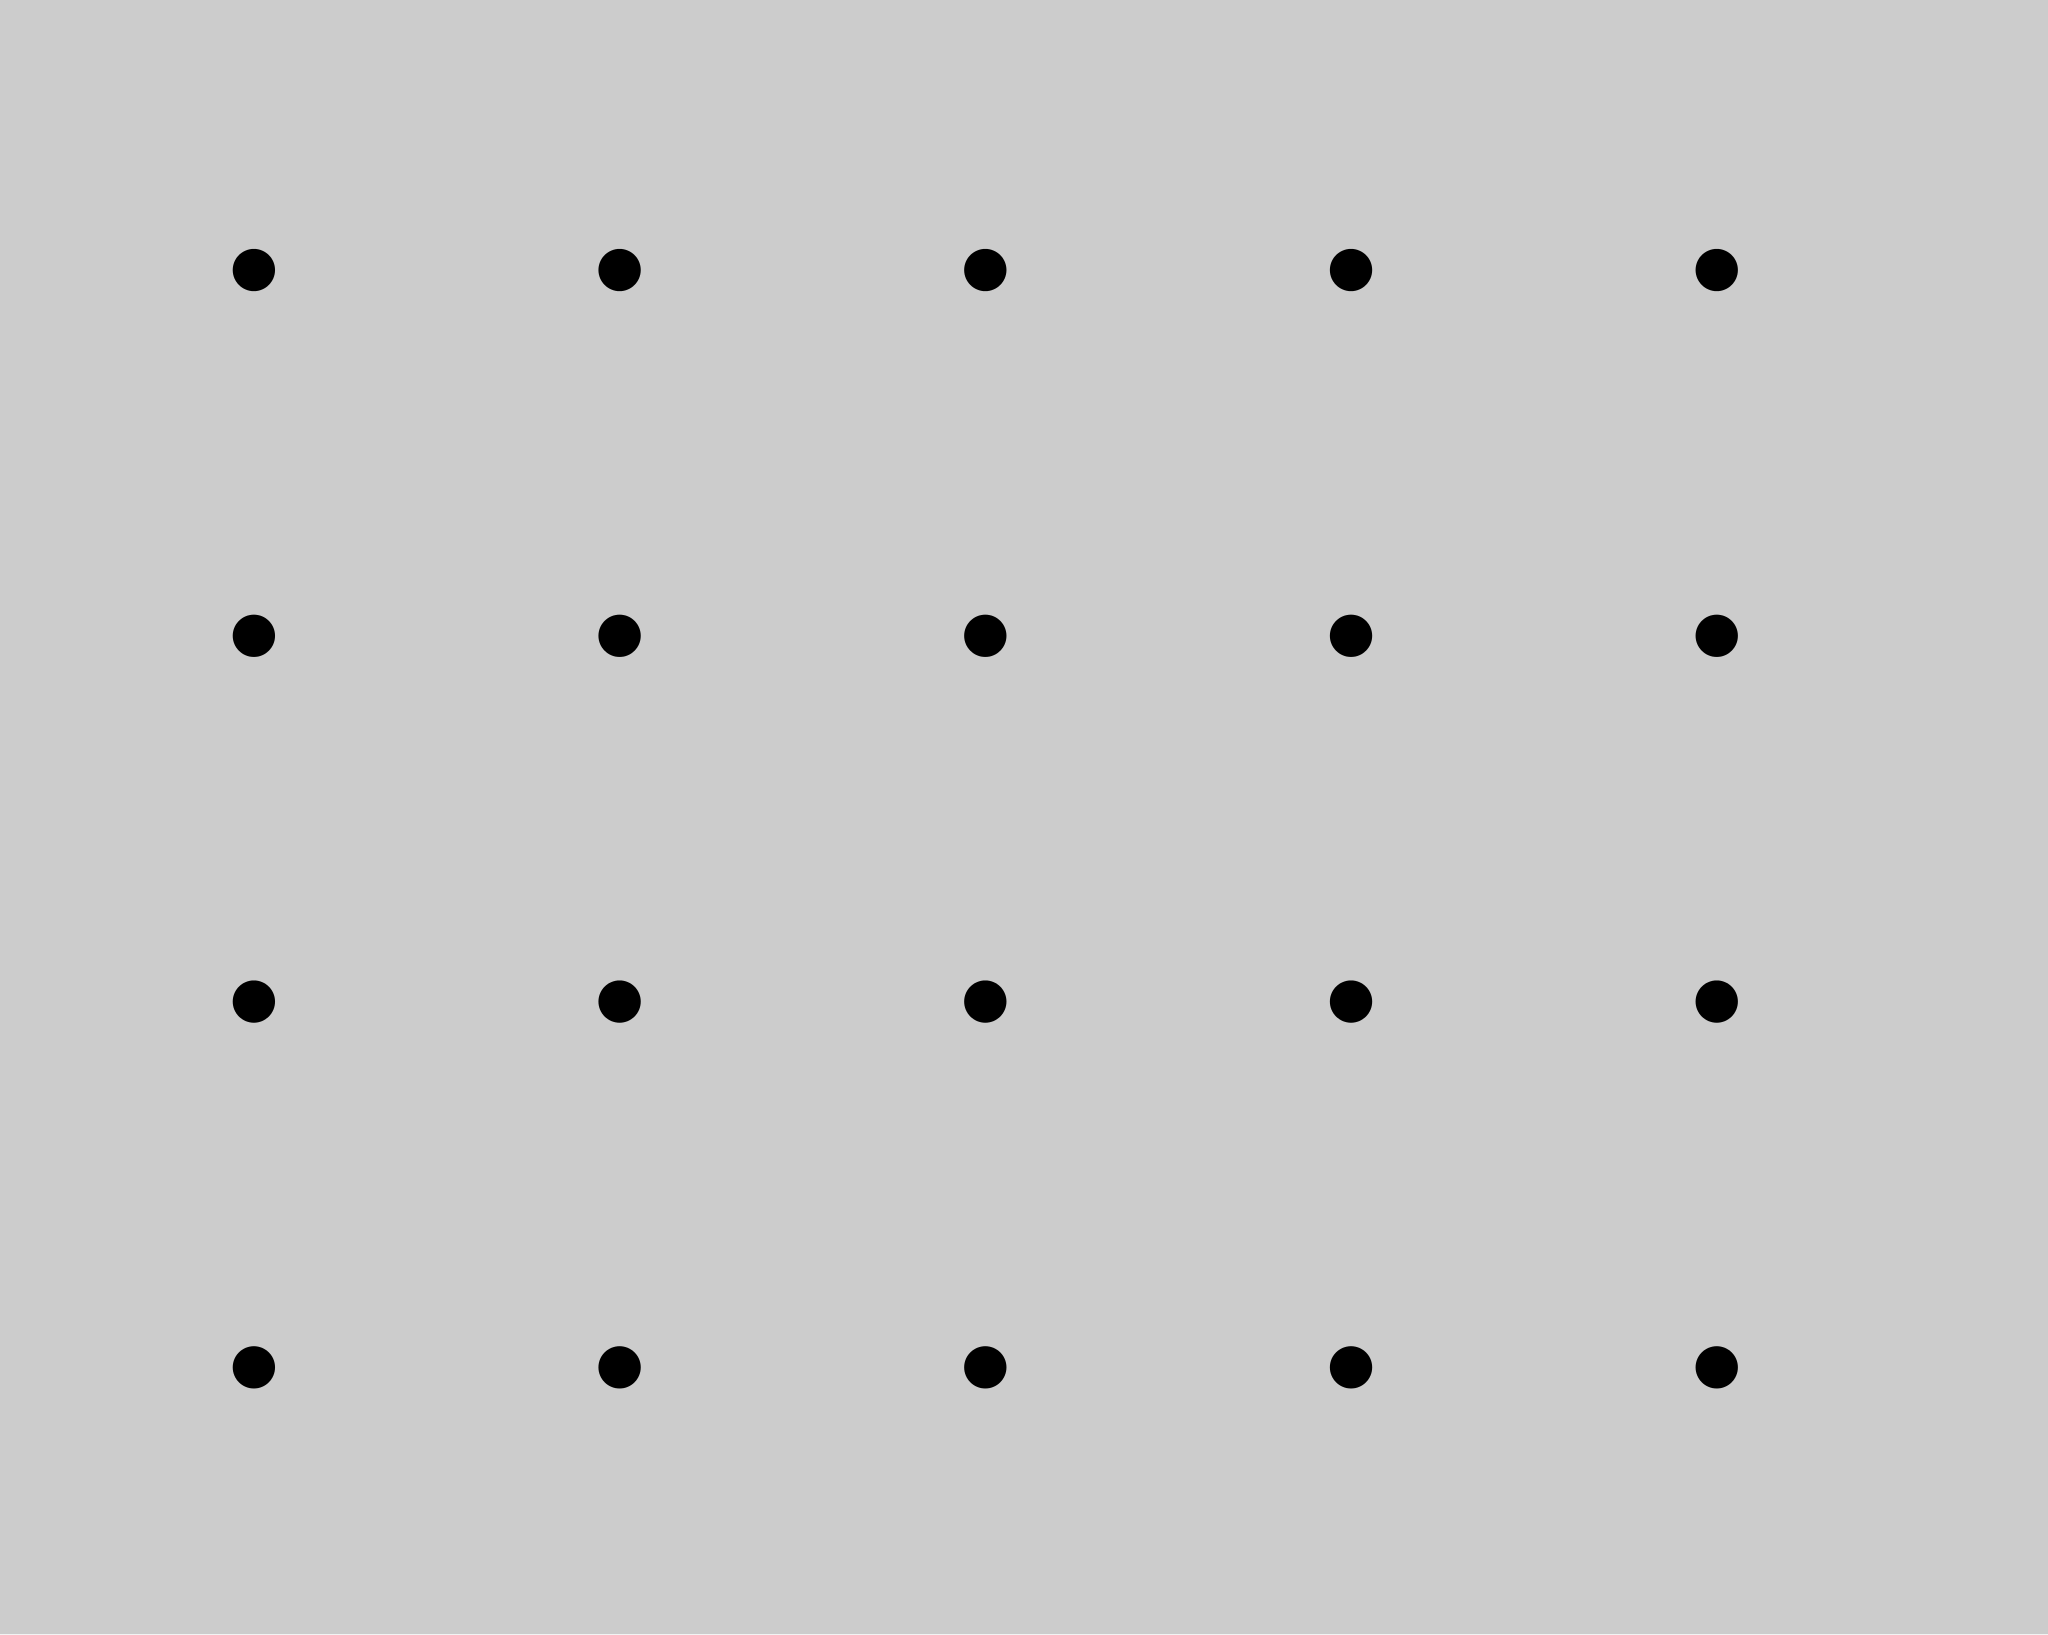
\includegraphics[width=100mm]{images/ch6_img03_ideal2d.png}
\caption{Ideale Verteilung von Elementen auf einer zweidimensionalen Fläche}
\label{img:ch6_img03_ideal2d}
\end{center}
\end{figure}

Für den Transfer der Kriterien auf den Anwendungsfall, muss berücksichtigt werden, dass die Spieler sich nicht per Luftlinie fortbewegen können. Diese können sich auf Grund der ortsbezogenen Affordanzen nur über die üblichen Wege fortbewegen. Diese Problematik betrifft auch die Fälle, in denen es geografische Hindernisse gibt. Beispielsweise wenn zwei Stadtteile zwar direkt nebeneinander liegen, diese aber durch einen Fluss getrennt sind. Diese Einschränkungen spiegeln sich alle im Wegnetz wieder. Daher muss untersucht werden, wie die optimale Verteilung der Spielelemente auf Basis der nächstgelegenen Wege stattfinden kann. Da die Punkte allerdings nicht selbst ausgewählt werden sondern aus OSM stammen und das Finden der besten Punkte ein zu komplexes Optimierungsproblem darstellen würde, muss ein anderer Ansatz verfolgt werden. Es ist somit notwendig die Abstände zwischen den einzelnen Spielelementen  zu bestimmen. Hierzu ist es notwendig die kürzeste Route zwischen zwei Punkten zu finden.
Da die meisten Routinglösungen reine Straßen bevorzugen, aber selten auch ausreichende Fußwege aufweisen, soll in diesem Fall wiederum auf OSM gesetzt werden.
Ziel soll es sein die Distanz zwischen den Spielelementen durch ein Offline Routing unter Verwendung von OSM zwischen den einzelnen Punkten zu bestimmen.
Zunächst muss aber bestimmt werden, welche der Spielelemente begutachtet werden. Hierfür werden dem entwickelten Evaluationstool jeweils ein OSM-Tag für die Auswahl der Spielelemente, sowie eine entsprechende Koordinate übergeben. Anhand dieser Information baut das Evaluationstool zwei Bounding Boxen. Diese werden unterschieden in die innere und äußere Bounding Box. Erstere enthält alle Punkte die untersucht werden sollen und letztere alle Punkte die zur Beurteilung herangezogen werden. Dieses Vorgehen ist nötigt, da ansonsten die Punkte an den Ecken der inneren Bounding Box bei einer Bewertung benachteiligt werden würden.
Die Anordnung der Bouding Boxen ist in Abbildung \ref{img:ch6_img04_bbox} zu sehen.
Die innere Bounding Box (schwarz) wurde im konkreten Fall auf 2,5km Breite und Länge 6,25km$^2$ festgesetzt. Im Gegensatz dazu steht die äußere Bounding Box (rot), welche um die innere um die maximale Evaluationsdistanz erweitert wurde. Im konkreten Fall soll diese Distanz 700 Meter darstellen, welches die Distanz von 10 Minuten Fußweg widerspiegelt. Die Wahl ist auf 10 Minuten gefallen um eine ausreichende Dichte der Spielfelder zu erreichen und die Spieler zudem zur Fortbewegung zu motivieren.


\begin{figure}[H]
\begin{center}
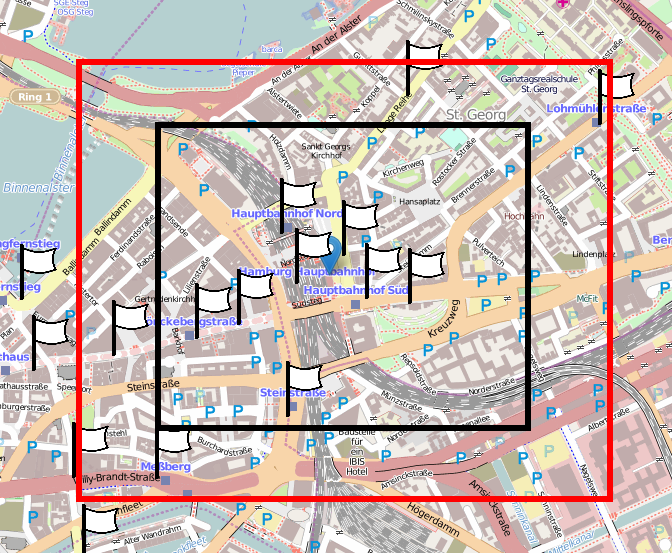
\includegraphics[width=100mm]{images/ch6_img04_bbox.png}
\caption{Inner und äußere Bounding Box zur Evaluation}
\label{img:ch6_img04_bbox}
\end{center}
\end{figure}

Zur Evaluation wurde eine Abwandlung der k-Nearest Neighbours Methode, konkret die count Nearest Neighbours gewählt.
Sie basiert auf der K-Funktion die in Kapitel \ref{ch3:s:geostatistik} von \textcite{Spooner.2004} vorgestellt wurde.
Es soll dabei nicht die Entfernung der 10 nächsten Spielelemente ausgelesen werden, sondern die Anzahl der Spielelemente die im  Umkreis von k Metern sind. Für die Evaluation wurde k auf 700 Meter festgelegt. Die Idee ist es eine Art geografische Dichte bestimmen zu können, welche eine Information für den Spielleiter darstellt.
Zunächst wurde die Idee eines zeitgeographischen Netzwerks verfolgt. Hierbei sollten ausgehend von einem Element alle Wege als Netzwerk aufgebaut werden, welche in den Umkreis von 700 Metern fallen. Nach der ersten Evaluation wurde eine durchschnittliche Zeit von 40 Sekunden gemessen für die Aufbereitung des Netzwerks. Die Prüfung ob ein Element auf den besagten Wege-Netzwerk liegt dagegen läuft in wenigen ms ab.
Im Anbetracht der verwendeten Tags, die im Schnitt 150 Elemente in der inneren Bounding box haben, sind dies für die Evaluation bereits 75 Minuten.
Soll dagegen eine ganze Liste von Tags überprüft werden, so steigt die Evaluationszeit für eine Koordinate mit mehreren Tags schnell auf mehrere Tage.
Aus diesem Grund wurde eine Alternative für die zeitaufwendige Methode gesucht.
Durch die Verwendung des Graphhopper-Tools ist es möglich ein sehr schnelles und effizientes Routing zwischen zwei Punkten durchzuführen.
Tests haben ergeben, dass eine Route unter 100ms ermittelt werden kann. Die Idee ist den logisch aufwändigeren Weg zu gehen und die Distanz zu allen bestehenden Punkten zu berechnen. Somit muss für jedes Element der inneren Bounding Box die Entfernung zu jedem Element innerhalb der äußeren Bounding Box bestimmt werden. Zwar nimmt die Laufzeit quadratisch zu im Vergleich zur zeitgeographischen Variante, jedoch liegt diese deutlich niedriger. Bei 167 inneren Elementen und 263 äußeren lag die Evaluationszeit pro Spielelement bei ca. 1,5 Sekunden. D.h. um den Faktor 26 kleiner als per zeitgeographisches Netzwerk. Dadurch ergibt sich ein Break Even Punkt an dem sinnvoller ist von der einfacheren Methode auf die zeitgeographische zu wechseln.
Dieser Punkt liegt, wie sich in Abbildung \ref{img:ch6_img05_eval_match} erkennen lässt, bei ungefähr 4100 Elementen.
Darüber hinaus wurde die Analyse der Tags parallelisiert um die volle Rechenkapazität des jeweiligen Rechners ausnutzen zu können und somit schneller zum Ergebnis zu kommen. Bei aktuellen 4-8 Kern Prozessoren findet eine nicht zu vernachlässigende Geschwindigkeitssteigerung statt.

\begin{figure}[H]
\begin{center}
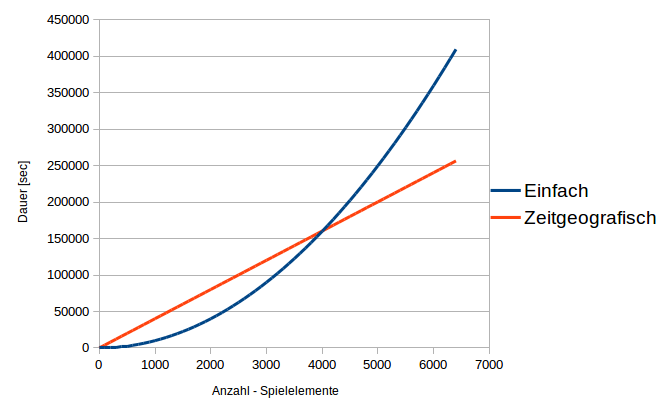
\includegraphics[width=150mm]{images/ch6_img05_eval_match.png}
\caption{Gegenüberstellung der cNN Methoden}
\label{img:ch6_img05_eval_match}
\end{center}
\end{figure}

Allerdings muss beachtet werden, dass bei 4100 Spielelementen auf 6,25km$^2$, eine extrem hohe Dichte erreicht wird. Diese führt dazu, dass es im Schnitt es weniger als 40 Meter bis zum nächsten Spielelement sind. Bei einem Aktionsradius von 40 Metern, wäre das Spielfeld somit voller Spielelemente. Daraus folgern sich zwei Dinge:
Die ideale Spielelementzahl sollte einen Flächen zu Spielemement Index größer als 1524m$^2$ aufweisen.
Es ist auch festzustellen, dass der Einsatz der zeitgeographische Methode keinen Sinn macht.
Nachdem die Berechnungsmethode festgelegt wurde und die Werte für verschiedene Punkte berechnet wurde, wurde festgestellt, dass ein Clustering sich nicht negativ auf die Ergebnisse auswirkt.
Der Grund hierfür liegt in der Bewertungsfunktion. Jedes Spielelement im Bereich von 0 bis 700 Meter wird als ein nächster Nachbar gezählt.
Die Ursprüngliche Vorgehensweise hatte als Bewertungsfunktion der einzelnen Tags:

\begin{equation}
score = \frac{ \sum\limits_{i=1}^n c_n }{n}
\end{equation}

Um dieses Problem zu umgehen muss eine Bewertungsfunktion für die unterschiedlichen Entfernungen erstellt werden. Ein erster Ansatz die Verwendung einer Gleichung zweiter Ordnung wie in Abbildung \ref{img:ch6_img06_valued2} zu erkennen. Nach einem ersten Probelauf hat sich allerdings herausgestellt, dass die Elemente im Bereich von unter 1000 Metern zu schwach negativ ins Gewicht fallen.

\begin{figure}[H]
\begin{center}
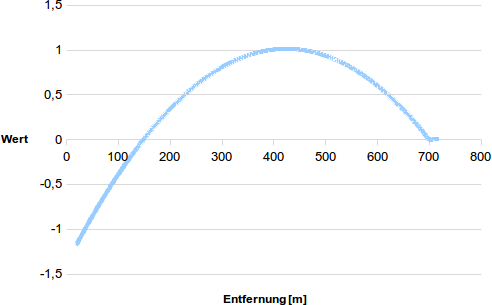
\includegraphics[width=150mm]{images/ch6_img06_valued2.png}
\caption{Bewertungsfunktion für Distanzen}
\label{img:ch6_img06_valued2}
\end{center}
\end{figure}

\begin{equation}
weighted score = \frac{ \sum\limits_{i=1}^n cv_n }{n}
\end{equation}

Aus diesem Grund wurde auf eine abgestufte Bewertung gewechselt, welche das Ergebnis für die entsprechenden Tags besser normalisiert hat.
Allerdings ist das Ergebnis welches in Abbildung \ref{img:ch6_img07_result1} zu sehen ist noch nicht das Optimum. Es wird daher vorgeschlagen, die Bewertungsfunktion weiter zu optimieren und Ansätze aus der Fuzzy Logic zu verfolgen, da diese eine deutlich bessere Steuerung der einzelnen Attribute und Entfernungen ermöglichen. Eine vollständige Grafik aller Werte ist im Anhang zu finden. Die in Abbildung \ref{img:ch6_img07_result1} gezeigte Darstellung zeigt die Tags die weniger als 70 Nachbar-Elemente im Umkreis von 700 Metern haben.
Es lässt sich erkennen, dass Elemente, welche durch die Infrastruktur bedingt verteilt gelegen sind wie z.B: Bushaltestellen, Bäckereien und Ampel eine bessere Verteilung haben als zum Beispiel Schulen. Allerdings muss beachtet werden, dass allein durch ein höheren Wert nicht sichergestellt ist, dass der Tag überall gut funktioniert. Viel wichtiger dabei ist der Abgleich der Werte aus verschiedenen Regionen. Erst mit dem Vergleich der Ergebnisse der einzelnen Tags an unterschiedlichen Orten, an denen ein Staging stattfinden soll, ermöglicht eine Auswahl.
Der Tag, welcher bei allen Überprüften Lokalitäten den ausgeglichensten Wert hat, sollte verwendet werden. Gibt es mehrere Tags die im Schnitt wenig voneinander Abweichen, sollte der Tag mit dem höchsten Wert verwendet werden. 

\begin{figure}[H]
\begin{center}
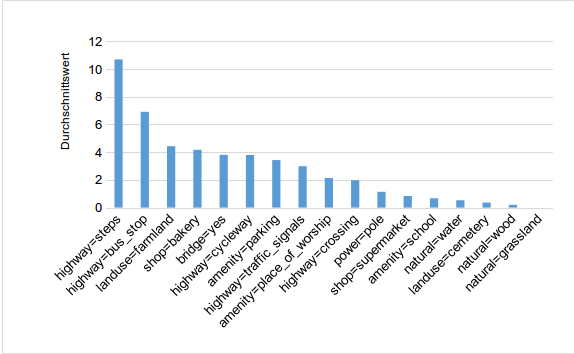
\includegraphics[width=150mm]{images/ch6_img07_result1.png}
\caption{Bewertung der verschiedenen Tags}
\label{img:ch6_img07_result1}
\end{center}
\end{figure}
